\begin{tikzpicture}

%A matrix
\draw [fill=cyan, opacity=.2,rotate=90, thick]  (0.1,5.05) node (v1) {} rectangle (3.9,-2.15) node (v2) {};
\draw [thick,rotate=90,red] (v1) rectangle (3.9,4);
\draw [thick,rotate=90,red] (0.1,4) rectangle (3.9,2.95) node (v7) {};
\draw [thick,rotate=90,red] (0.1,-1) node (v6) {} rectangle (v2);
\draw[thick,red]  (v6) rectangle (-0.15,3.9);
\draw[thick,red,fill=orange, opacity=0.6]  (v7) rectangle (-1.9,0.1);

\node at (-5.65,1.6) { \color{blue}\Large  \bf  \vdots};
\node  at (-5.65,3.6) {\color{blue} \bf  \huge $\underline{a_1}$};
\node at (-5.65,2.6) { \color{blue} \bf  \huge $\underline{a_2}$};
\node at (-5.65,0.6) {\color{blue} \bf  \huge $\underline{a_m}$};
\node at (-1.65,-1.4) {\huge$ \underset{ \color{blue} ( m \ll n)}{A_{ m \times n} }$};

% X vector
\draw [ thick, fill=green] (5.85,5) rectangle (6.85,6);
\draw [thick] (6.85,5) rectangle (5.85,4);
\draw [thick, fill=green] (5.85,4) rectangle (6.85,3);
\draw [] (5.85,3) node (v4) {} rectangle (6.85,-0.1) node (v5) {};
\draw [thick] (5.85,-0.1) rectangle (6.85,-1.1);
\draw [thick, fill=green] (5.85,-1.1) rectangle (6.85,-2.1);
\node at (6.45,-3.4) {\huge $\underset{\tiny \color{blue} (K-sparse)}{x_{n \times 1 }} $};
\node at (6.35,1.6) {\Large \bf \vdots};
\node at (3.25,2.1) {\Huge $\times$};
\draw [thick] (v4) rectangle (6.85,2.1);
\draw [thick] (v5) rectangle (5.85,0.8);

% delta-x vector
\draw [ thick] (9.55,5) rectangle (10.55,6);
\draw [thick] (10.55,5) rectangle (9.55,4);
\draw [thick, fill=orange] (9.55,4) rectangle (10.55,3);
\draw [] (9.55,3) node (v4) {} rectangle (10.55,-0.1) node (v5) {};
\draw [thick] (9.55,-0.1) rectangle (10.55,-1.1);
\draw [thick] (9.55,-1.1) rectangle (10.55,-2.1);
\node at (10.15,-3.4) {\huge $\underset{\tiny \color{blue} (increment)}{\Delta_{i}} $};
\node at (10.05,1.6) {\Large \bf \vdots};
\node at (3.25,2.1) {\Huge $\times$};
\draw [thick] (v4) rectangle (10.55,2.1);
\draw [thick] (v5) rectangle (9.55,0.8);

\node at (8.25,2) {\Huge \bf $+$};
\node at (10.05,3.5) {\huge $k$};

% y

\draw [thick] (17.75,4.1) node (v3) {} rectangle (18.75,3.1);
\draw [thick] (17.75,3.1) rectangle (18.75,2.1);
\draw [thick] (17.75,2.1) rectangle (18.75,1);
\draw [thick] (17.75,1) rectangle (18.75,0);
\draw[fill=orange,opacity=0.6]  (v3) rectangle (18.75,0);

\node at (15.25,1.6) {\bf \vdots};

\node at (13.1,2) {\Huge = };
\node at (15.35,-1.2) {\huge $ \underset{ \color{blue} (sketch \ of \ x) }{y_{m \times 1}}$};

\node at (-1,2.5) {\Huge \bf $\cdots$};



% b_k

\draw [thick] (14.75,4.1) node (v3) {} rectangle (15.75,3.1);
\draw [thick] (14.75,3.1) rectangle (15.75,2.1);
\draw [thick] (14.75,2.1) rectangle (15.75,1);
\draw [thick] (14.75,1) rectangle (15.75,0);
\draw[fill=red, opacity=0.2]  (v3) rectangle (15.75,0);
\node at (-2.5,1.6) { \color{blue}\Large  \bf  \vdots};


\node at (18.2,1.6) {\bf \vdots};

\node at (18.35,-1.2) {\huge $ \underset{ \color{blue} (update) }{b_k}$};



\node at (-3.45,2.5) {\large \bf $\cdots$};
%\draw [dashed,blue] (-5.05,3.9) rectangle (2.15,3);
\draw [dashed,blue] (-5.05,3) rectangle (2.15,2);
\draw[dashed,blue]  (v1) rectangle (2.15,1);
\node at (-4.6,4.5) {\huge \bf  \color{red} $b_0$};
\node at (-3.45,4.5) {\huge \bf \color{red} $\cdots$};
\node at (-2.45,4.5) {\huge \bf  \color{red} $b_k$};
\node at (-0.95,4.5) {\huge \bf  \color{red} $\cdots$};
\node at (0.55,4.5) {\huge \bf  \color{red} $b_{n-1}$};
\node at (1.65,4.5) {\huge \bf  \color{red} $b_n$};
\draw (4.7031,5.2202) arc (160:200:10);

\node at (10.05,4.55) {\large \bf \vdots};
\draw (11.5668,5.5912) arc (19.9999:-20:10.5);
\node at (16.7,2) {\Huge \bf $+$};
\end{tikzpicture}